\section{Пошук відповідності між кадрами}

Рух камери не є рідкістю для відеозаписів лекцій. Камера може труситись,
коли її прикріплено до столу, де студенти пишуть лекцію, або від
вібрацій полу, коли викладач ходить по ньому. Камеру може рухати
оператор для того, щоб сфокусувати увагу глядачів на певному сегменті
дошки. У даному розділі описано оцінку гомографії за допомогою
дескриптора ознак SIFT, як одного з кроків вирішення вищеописаних
проблем.

Оскільки дошка вважається плоскою поверхнею, побудувати відповідність
між точками дошки на різних зображеннях можна за допомогою гомографії.
Рухи камери під час лекції можуть змінюватися від незначних
субпіксельних зсувів до зміщень, в результаті яких видимою стає частина
дошки, яка до цього була прихованою. Наша мета -- зробити слайди, де
камера виглядає статичною, а сегменти дошки поступово стають видимими та 
поєднуються для утворення панорами.

Ми можемо використовувати дескриптори ознак, такі як SIFT, SURF [13] або ORB
[14], щоб знайти ключові точки (feature points). Був обраний SIFT, оскільки під час
експериментів він надав візуально кращі результати, ніж інші алгоритми.


\subsection{SIFT}

У 1999 році англієць Девід Лоу представив алгоритм SIFT (Scale-invariant feature transform) 
% \cite{Lowe_david_2004}
,укр. \textit{Масштабозалежне перетворення ознак}. Даний алгоритм 
застовуэться для знаходження ключових точок (локальних ознак) зображення. Метод досить точно 
і швидко знаходить дані точки.
Головною перевагою алгоритму є інваріантність щодо просторової орієнтації та якості освітлення.
Має широке застосування в області комп'ютерного зору як один з кроків для побудови 3D-карт, 
ректифікації стереопар та детектингу об'єктів.

Коротко розпишемо структуру алгоритму.

\begin{enumerate}
    \item \textbf{Пошук масштабно-просторових екстремумів}
        На даному етапі потрібно знайти зони зображення та такі масштаби, які можна повторно 
        знайти при різних перспективах(точок погляду). Тут використовується просторово та 
        масштабно інваріантне ядро оператора Гауса з операцією конволюції 
        до зображення $L(x,y,\sigma) = G(x,y,\sigma) \ast I(x,y)$, 
        де $G(x,y,\sigma) = (1/2\pi\sigma^2)\exp({-(x^2+y^2)/2\sigma^2})$.


        Будується різниця гаусіан (DoG метод) з константою $k$:

        \begin{equation}
            D(x,y,\sigma) = (L(x,y,k\sigma) - L(x,y,\sigma))
        %  \cite{}
        \end{equation}

        Тобто початкове зображення поступово піддається конволюціям гаусианів з константою
        $k$ на кожну епоху. При чому кожна епоха відрізняється між собою значенням $k = 2^{1/s}$,
        де $s$ число, що показує на скільки інтервалів розділити кожну епоху.
        В стеку однієї епохи зберігається $s+3$ зображень. Коли епоха завершиться, то
        створюється нове Гаусове зображення з двох найвищих в стеку,
        взяттям кожного 2-го пікселя рядка і колонки.  

        \begin{figure}[H]
            \centering
            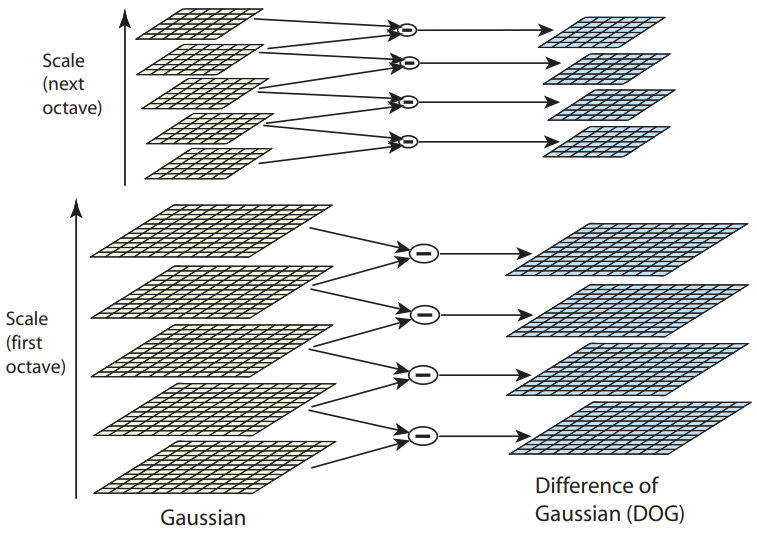
\includegraphics[width=0.6\textwidth]{images/sift1}
            \caption{Знаходження різниць гаусианів 1-го етапу SIFT}
            \label{fig:swift1}
        \end{figure}

        \subitem \textbf{Пошук локальних екстремумів} \\
                Для знаходження локальних екстремумів зображення різниці гауссіан 
                якоїсь точки беруться 8 сусідів цього ж зображення і 9 зображення різниць 
                зверху та знизу. Точка є екстремум якщо вона значення її більше або менше за 
                значення всіх її сусідів.

                \begin{figure}[H]
                    \centering
                    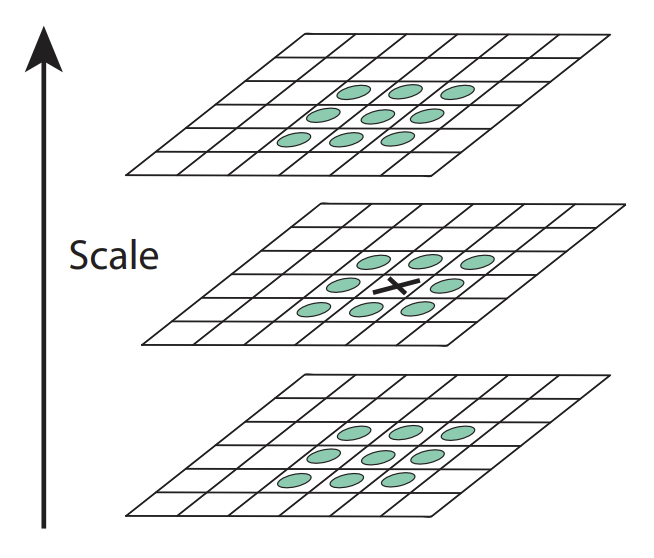
\includegraphics[width=0.3\textwidth]{images/sift2}
                    \caption{Знаходження різниць гаусианів 1-го етапу SIFT}
                    \label{fig:swift2}
                \end{figure}

        \subitem \textbf{Частота вибірки по масштабу} \\
                Тут автор обґрунтовує кількість того, скільки разів потрібно робити 
                зміну масштабу зображення. Експерименти показують, що на даному етапі метод дає
                велику кількість кандидатів екстремумів, і що це дуже важко обрахувати їх всі.
                \begin{figure}[H]
                    \centering
                    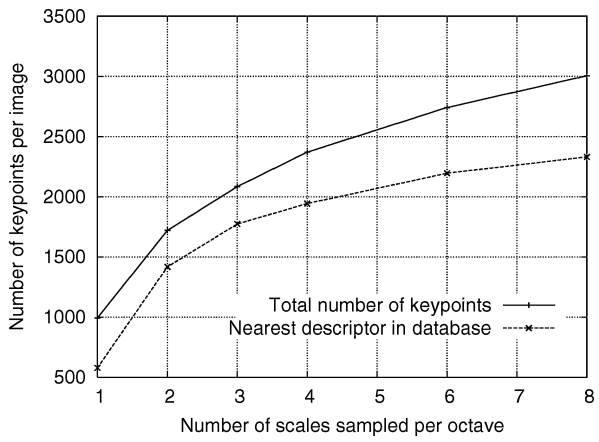
\includegraphics[width=0.4\textwidth]{images/sift3}
                    \caption{Графік залежності кількості змін масштабу на кожну епоху до 
                            кількості ключових точок на зображенні}
                    \label{fig:swift3}
                \end{figure}

        \subitem \textbf{Частота вибірки по простору} \\
                Пропонується використовувати оптимальне значення $\sigma = 1.6$ при якому 
                маємо найбільший відсоток співпадіння екстремумів при багатократному повторенні
                експерименту.

    \item \textbf{Точна локалізація ключових точок}
        Після знаходження точок-кандидатів потрібно відсіяти точки зі слабким контрастом на основі
        інформації масштабів та відношення головних викривлень. Для цього застосовується рокзклад
        Тейлора масштабно-просторової функції $D(x,y,\sigma)$ в точці $\textbf{x} = (x,y,\sigma)$.
        \begin{equation}
            D(\textbf{x}) = D + \frac{\partial D^T }{\partial \textbf{x} }\textbf{x} + 
                       \frac{1}{2}\textbf{x}^T\frac{\partial^2 D}{\partial \textbf{x}^2}\textbf{x}
            \label{eq:tailor_1}
        \end{equation}
        Місце де знаходиться екстремум $\widehat{\textbf{x}}$:
        \begin{equation}
            \widehat{\textbf{x}} = \frac{\partial^2 D^{-1} }{\partial
                                    \textbf{x}^2}\frac{\partial D }{\partial \textbf{x}}
            \label{eq:extremum}
        \end{equation}
        Підставивши \ref{eq:extremum} у  \ref{eq:tailor_1} маємо можлвість відсіяти нестабільні
        екстремуми по модулю значення (рис. \ref{fig:sift45}):
        \begin{equation}
            D(\widehat{\textbf{x}}) = D + \frac{1}{2}\frac{\partial D^{T} }{\partial \textbf{x}}\widehat{\textbf{x}}
        \end{equation}

        \begin{figure}[H]
            \centering
            \ContinuedFloat
            \begin{subfigure}[c]{0.3\textwidth}
                \centering
                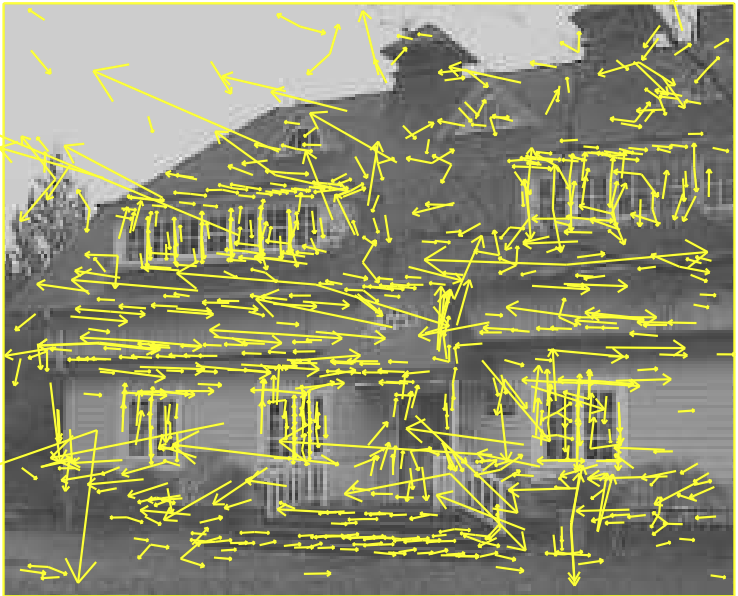
\includegraphics[width=\textwidth]{images/sift4}
                \caption{ 832 ключових точок
                \label{fig:swift4}
                }
            \end{subfigure}
            \begin{subfigure}[c]{0.3\textwidth}
                \centering
                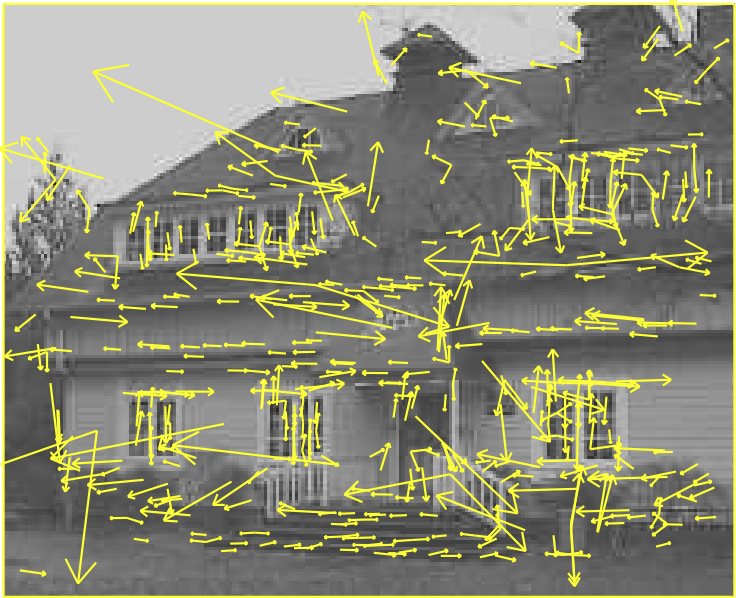
\includegraphics[width=\textwidth]{images/sift5}
                \caption{ 536 ключових точок
                \label{fig:swift5}
                }
            \end{subfigure}
            \caption{Приклад відсіювання екстремумів
            \label{fig:sift45}
            }
        \end{figure}
        Тобто обмежуючи $|D(\widehat{\textbf{x}})| < \alpha$. Якщо кожен піксел в діапазоні $[0,1]$, то і 
        $ \alpha \in [0,1]$.
    \item \textbf{Визначення орієнтації градієнтів} \\
        До кожної точки визначаэться декілька орієнтацій градієнтів.
        Магнітуда градієнта по сусідам $m(x,y)$ та його орієнтація $\theta(x,y)$:
        \begin{equation}
            m(x,y) = \sqrt{(L(x+1,y) - (L(x-1,y))^2 + (L(x,y+1) - L(x,y-1))^2}
        \end{equation}
        \begin{equation}
        \theta(x,y) = \tan^{-1} (L(x,y+1) - L(x,y-1))/(L(x+1,y) - L(x-1,y))
        \end{equation}
        , де $L(x,y)$ - значення згладженого гаусового зображення з найближчим масштабом.

    \item \textbf{Дескриптор точок} \\
        Локальні градієнти обчислюються для кожного масштабу навколо кожної ключової точки.
        Створюються дескриптори кожної ключової точки.
        \begin{figure}[H]
            \centering
            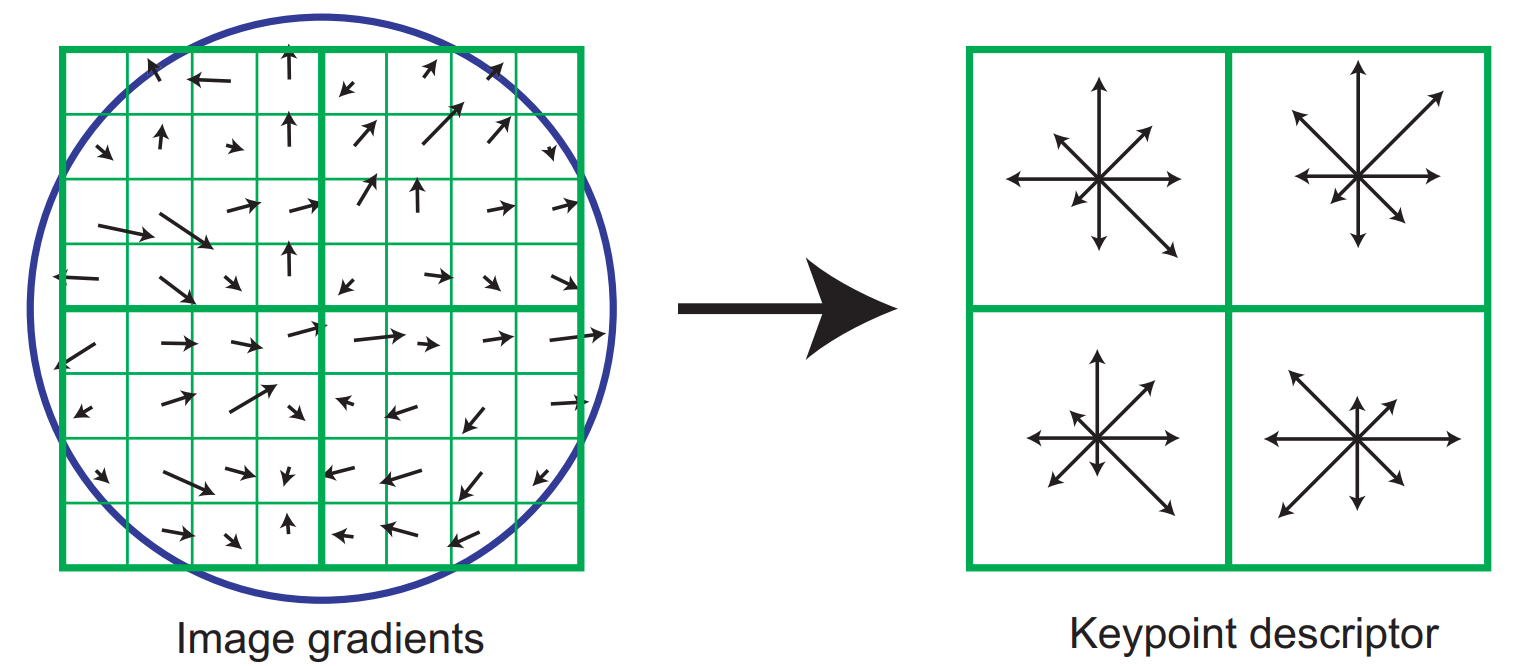
\includegraphics[width=0.5\textwidth]{images/sift6}
            \caption{Створення дескрипторів точок}
            \label{fig:swift6}
        \end{figure}
\end{enumerate}